\chapter{Specifikacija programske potpore}
		
	\section{Funkcionalni zahtjevi}
			
			\textbf{\textit{dio 1. revizije}}\\
			
			\textit{Navesti \textbf{dionike} koji imaju \textbf{interes u ovom sustavu} ili  \textbf{su nositelji odgovornosti}. To su prije svega korisnici, ali i administratori sustava, naručitelji, razvojni tim.}\\
				
			\textit{Navesti \textbf{aktore} koji izravno \textbf{koriste} ili \textbf{komuniciraju sa sustavom}. Oni mogu imati inicijatorsku ulogu, tj. započinju određene procese u sustavu ili samo sudioničku ulogu, tj. obavljaju određeni posao. Za svakog aktora navesti funkcionalne zahtjeve koji se na njega odnose.}\\
			
			
			\noindent \textbf{Dionici:}
			
			\begin{packed_enum}
				
				\item Vlasnik (naručitelj)
				\item Vlasnik psa
				\item Vlasnik obrta
				\item Razvojni tim
				
			\end{packed_enum}
			
			\noindent \textbf{Aktori i njihovi funkcionalni zahtjevi:}
			
			
			\begin{packed_enum}
				\item  \underbar{Neregistrirani/neprijavljeni korisnik može:}
				
				\begin{packed_enum}
					
					\item pregledati lokacije na karti
					\item odabrati lokaciju i dobiti prikaz opcih informacija (ime lokacije, adresa, telefon, OIB, kratak opis, djelatnost)
					\item se registrirati u sustav, stvoriti novi korisnicki račun za koji su mu potrebni korisničko ime, lozinka, ime, prezime, broj mobitela, e-mail adresa
					
					
				\end{packed_enum}
			
				\item  \underbar{Registirani korisnik može:}
				
				\begin{packed_enum}
					
					\item pregledavati i mijenjati osobne podatke
					\item izbrisati svoj korisnički račun
					\item pisati recenzije i dati ocjene
					\item pregledati recenzije
					
				\end{packed_enum}
				
			
				\item  \underbar{Baza podataka(sudionik):}
				
				\begin{packed_enum}
					
					\item pohranjuje sve podatke o korisnicima i njihovim ovlastima
					\item pohranjuje sve podatke o lokacijama

					
				\end{packed_enum}
				
			\end{packed_enum}
			
			\eject 
			
			
				
			\subsection{Obrasci uporabe}
				
				\textbf{\textit{dio 1. revizije}}
				
				\subsubsection{Opis obrazaca uporabe}
					\textit{Funkcionalne zahtjeve razraditi u obliku obrazaca uporabe. Svaki obrazac je potrebno razraditi prema donjem predlošku. Ukoliko u nekom koraku može doći do odstupanja, potrebno je to odstupanje opisati i po mogućnosti ponuditi rješenje kojim bi se tijek obrasca vratio na osnovni tijek.}\\
					

					\noindent \underbar{\textbf{UC1 - Pregled lokacija na karti}}
					\begin{packed_item}
	
						\item \textbf{Glavni sudionik: }Registrirani korisnik, Neregistrirani korisnik
						\item  \textbf{Cilj:} Pregledati lokacije i osnovne informacije
						\item  \textbf{Sudionici:} Baza podataka, Google Maps API
						\item  \textbf{Preduvjet:} -
						\item  \textbf{Opis osnovnog tijeka:}
						
						\item[] \begin{packed_enum}
	
							\item Karta je prikazana prilikom učitavanja aplikacije
							\item Korisnik na karti odabire lokaciju
							\item Prikazuju se informacije o lokaciji i ponudi

						\end{packed_enum}
						
					\end{packed_item}
					
					\noindent \underbar{\textbf{UC2 - Registracija  obrta}}
					\begin{packed_item}
	
						\item \textbf{Glavni sudionik: }Neregistrirani korisnik
						\item  \textbf{Cilj:} Stvoriti korisnički račun za pristup sustavu
						\item  \textbf{Sudionici:} Baza podataka
						\item  \textbf{Preduvjet:} -
						\item  \textbf{Opis osnovnog tijeka:}
						
						\item[] \begin{packed_enum}
	
							\item Korisnik odabire opciju za registraciju
							\item Korisnik odabire opciju "Company"
							\item Korisnik unosi podatke
							\item Korisnik prima e-mail za potvrdu registracije
							\item Korisnik potvrđuje registraciju
							\item Prikazuje se poruka o uspješnoj registraciji

						\end{packed_enum}
						
						\item  \textbf{Opis mogućih odstupanja:}
						
						\item[] \begin{packed_item}
	
							\item[2.a] Odabir već zauzetog korisničkog imena i/ili e-maila, unos korisničkih podataka u nedozvoljenom formatu ili pružanje neispravnog e-maila, ne zadovoljavanje kompleksnosti lozinke
							\item[] \begin{packed_enum}
								
								\item Sustav obavještava korisnika o neuspješnom upisu i vraća ga na stranicu za registraciju
								\item Korisnik mijenja podatke te završava unos ili odustaje od registracije
								
							\end{packed_enum}
							
						\end{packed_item}
					\end{packed_item}
					
					\noindent \underbar{\textbf{UC3 - Registracija privatne osobe}}
					\begin{packed_item}
	
						\item \textbf{Glavni sudionik: }Neregistrirani korisnik
						\item  \textbf{Cilj:} Stvoriti korisnički račun za pristup sustavu
						\item  \textbf{Sudionici:} Baza podataka
						\item  \textbf{Preduvjet:} -
						\item  \textbf{Opis osnovnog tijeka:}
						
						\item[] \begin{packed_enum}
	
							\item Korisnik odabire opciju za registraciju
							\item Korisnik odabire opciju "personal"
							\item Korisnik unosi podatke
							\item Korisnik prima e-mail za potvrdu registracije
							\item Korisnik potvrđuje registraciju
							\item Prikazuje se poruka o uspješnoj registraciji

						\end{packed_enum}
						
						\item  \textbf{Opis mogućih odstupanja:}
						
						\item[] \begin{packed_item}
	
							\item[2.a] Odabir već zauzetog korisničkog imena i/ili e-maila, unos korisničkih podataka u nedozvoljenom formatu ili pružanje neispravnog e-maila, ne zadovoljavanje kompleksnosti lozinke
							\item[] \begin{packed_enum}
								
								\item Sustav obavještava korisnika o neuspjelom upisu i vraća ga na stranicu za registraciju
								\item Korisnik mijenja podatke te završava unos ili odustaje od registracije
								
							\end{packed_enum}
							
						\end{packed_item}
					\end{packed_item}
					
					\noindent \underbar{\textbf{UC4 - Prijava u sustav}}
					\begin{packed_item}
	
						\item \textbf{Glavni sudionik: } Registrirani korisnik
						\item  \textbf{Cilj:} Dobiti pristup korisničkom sučelju
						\item  \textbf{Sudionici:} Baza podataka
						\item  \textbf{Preduvjet:} Registracija
						\item  \textbf{Opis osnovnog tijeka:}
						
						\item[] \begin{packed_enum}
	
							\item Unos e-maila i lozinke
							\item Potvrda ispravnosti unesenih podataka
							\item Pristup korisničkim funkcijama

						\end{packed_enum}
						
						\item  \textbf{Opis mogućih odstupanja:}
						
						\item[] \begin{packed_item}
	
							\item[2.a] Neispravno korisničko ime/lozinka
							\item[] \begin{packed_enum}
								
								\item Sustav obavještava korisnika o neuspjelom upisu i vraća ga na stranicu za prijavu
								
							\end{packed_enum}

						\end{packed_item}
					\end{packed_item}
					
					\noindent \underbar{\textbf{U5 - Pregled osobnih podataka}}
					\begin{packed_item}
	
						\item \textbf{Glavni sudionik: } Registrirani korisnik
						\item  \textbf{Cilj:} Pregledati osobne podatke
						\item  \textbf{Sudionici:} Baza podataka
						\item  \textbf{Preduvjet:} Korisnik je prijavljen
						\item  \textbf{Opis osnovnog tijeka:}
						
						\item[] \begin{packed_enum}
	
							\item Korisnik odabire opciju "Osobni podatci"
							\item Aplikacija prikazuje osobne podatke korisnika

						\end{packed_enum}
						
						
					\end{packed_item}
					
					\noindent \underbar{\textbf{UC6 - Promjena osobnih podataka}}
					\begin{packed_item}
	
						\item \textbf{Glavni sudionik: } Registrirani korisnik
						\item  \textbf{Cilj:} Promijeniti osobne podatke
						\item  \textbf{Sudionici:} Baza podataka
						\item  \textbf{Preduvjet:} Korisnik je prijavljen
						\item  \textbf{Opis osnovnog tijeka:}
						
						\item[] \begin{packed_enum}
	
							\item Korisnik odabire opciju za promjenu podataka
							\item Korisnik mijenja svoje osobne podatke
							\item Korisnik sprema promjene
							\item Baza podataka se ažurira

						\end{packed_enum}
						
						\item  \textbf{Opis mogućih odstupanja:}
						
						\item[] \begin{packed_item}
	
							\item[2.a] Korisnik promjeni svoje osobne podatke, ali ne odabere opciju "Spremi promjenu"
							\item[] \begin{packed_enum}
								
								\item Sustav obavještava korisnika da nije spremio podatke prije izlaska iz prozora

							\end{packed_enum}
							\item[2.b] Odabir već zauzetog korisničkog imena i/ili e-maila, unos korisničkog podatka u nedozvoljenom formatu ili pružanje neispravnog e-maila, ne zadovoljavanje kompleksnosti lozinke, promijenjena lozinka je jednaka trenutnoj
							\item[] \begin{packed_enum}
								
								\item Sustav obavještava korisnika o neuspjelom upisu i vraća ga na stranicu za promjenu podataka
								\item Korisnik mijenja podatke te završava unos ili odustaje od promjene podataka
								
							\end{packed_enum}
							
							
						\end{packed_item}
					\end{packed_item}
					
					\noindent \underbar{\textbf{UC7 - Brisanje korisničkog računa}}
					\begin{packed_item}
	
						\item \textbf{Glavni sudionik: } Registrirani korisnik
						\item  \textbf{Cilj:} Izbrisati svoj korisnički račun
						\item  \textbf{Sudionici:} Baza podataka
						\item  \textbf{Preduvjet:} Korisnik je prijavljen
						\item  \textbf{Opis osnovnog tijeka:}
						
						\item[] \begin{packed_enum}
	
							\item Otvara se stranica s osobnim podacima korisnika
							\item Korisnik briše račun
							\item Korisnički račun se izbriše iz baze podataka
							\item Otvara se stranica za registraciju

						\end{packed_enum}
						
						
					\end{packed_item}
					
					\noindent \underbar{\textbf{UC8 - Pregled informacija o lokaciji}}
					\begin{packed_item}
	
						\item \textbf{Glavni sudionik: }Registrirani/Neregistrirani korisnik
						\item  \textbf{Cilj:} Pregledati detaljnije informacije o lokaciji
						\item  \textbf{Sudionici:} Baza podataka, Google Maps API
						\item  \textbf{Preduvjet:} -
						\item  \textbf{Opis osnovnog tijeka:}
						
						\item[] \begin{packed_enum}
	
							\item Korisnik odabire određenu lokaciju
							\item Prikazuju se detaljne informacije o lokaciji

						\end{packed_enum}
						
					\end{packed_item}
					
					\noindent \underbar{\textbf{UC9 - Pregled informacija o obrtu}}
					\begin{packed_item}
	
						\item \textbf{Glavni sudionik: }Registrirani/Neregistrirani korisnik
						\item  \textbf{Cilj:} Pregledati detaljnije informacije o obrtu
						\item  \textbf{Sudionici:} Baza podataka, Google Maps API
						\item  \textbf{Preduvjet:} -
						\item  \textbf{Opis osnovnog tijeka:}
						
						\item[] \begin{packed_enum}
	
							\item Korisnik odabire određeni obrt
							\item Prikazuju se detaljne informacije o tom obrtu

						\end{packed_enum}
						
					\end{packed_item}
					
					\noindent \underbar{\textbf{UC10 - Filtriranje lokacije prema kategoriji}}
					\begin{packed_item}
	
						\item \textbf{Glavni sudionik: }Registrirani/Neregistrirani korisnik
						\item  \textbf{Cilj:} Filtrirati prikazane lokacije
						\item  \textbf{Sudionici:} Baza podataka, Google Maps API
						\item  \textbf{Preduvjet:} -
						\item  \textbf{Opis osnovnog tijeka:}
						
						\item[] \begin{packed_enum}
	
							\item Karta je prikazana prilikom učitavanja aplikacije
							\item Korisnik odabire željene kategorije
							\item Prikazuju se samo lokacije koje odgovaraju unesenim kategorijama

						\end{packed_enum}
						
					\end{packed_item}
					
					\noindent \underbar{\textbf{UC11 - Filtriranje lokacije prema unosu u polje za pretraživanje}}
					\begin{packed_item}
	
						\item \textbf{Glavni sudionik: }Registrirani/Neregistrirani korisnik
						\item  \textbf{Cilj:} Filtrirati prikazane lokacije
						\item  \textbf{Sudionici:} Baza podataka, Google Maps API
						\item  \textbf{Preduvjet:} -
						\item  \textbf{Opis osnovnog tijeka:}
						
						\item[] \begin{packed_enum}
	
							\item Karta je prikazana prilikom učitavanja aplikacije
							\item Korisnik unosi željeni tekst u polje za pretraživanje
							\item Prikazuju se samo lokacije koje odgovaraju unesenom tekstu

						\end{packed_enum}
						
					\end{packed_item}
					
					\noindent \underbar{\textbf{UC12 - Dohvaćanje lokacije uređaja}}
					\begin{packed_item}
	
						\item \textbf{Glavni sudionik: }Registrirani/Neregistrirani korisnik
						\item  \textbf{Cilj:} Prikazati točnu lokaciju korisnika
						\item  \textbf{Sudionici:} Google Maps API
						\item  \textbf{Preduvjet:} Prihvaćena privola za dohvaćanje lokacije uređaja
						\item  \textbf{Opis osnovnog tijeka:}
						
						\item[] \begin{packed_enum}
	
							\item Karta je prikazana prilikom učitavanja aplikacije
							\item Traži se privola korisnika
							\item Prikazuje se točna lokacija uređaja

						\end{packed_enum}
						
						\item  \textbf{Opis mogućih odstupanja:}
						
						\item[] \begin{packed_item}
	
							\item[2.a] Korisnik ne daje privolu
							\item[] \begin{packed_enum}
								
								\item Ne prikazuje se korisnikova lokacija
								
							\end{packed_enum}
							
						\end{packed_item}
						
					\end{packed_item}
					
					\noindent \underbar{\textbf{UC13 - Privola za dohvaćanje lokacije uređaja}}
					\begin{packed_item}
	
						\item \textbf{Glavni sudionik: }Registrirani/Neregistrirani korisnik
						\item  \textbf{Cilj:} Dobiti od korisnika dozvolu za lociranje
						\item  \textbf{Sudionici:} Google Maps API
						\item  \textbf{Preduvjet:} -
						\item  \textbf{Opis osnovnog tijeka:}
						
						\item[] \begin{packed_enum}
	
							\item Prikazuje se prozor u kojem se od korisnika traži dopuštenje
							\item Korisnik daje dopuštenje
							\item Prikazuje se točna lokacija uređaja

						\end{packed_enum}
						
						\item  \textbf{Opis mogućih odstupanja:}
						
						\item[] \begin{packed_item}
	
							\item[2.a] Korisnik ne daje privolu
							\item[] \begin{packed_enum}
								
								\item Ne prikazuje se korisnikova lokacija
								
							\end{packed_enum}
							
						\end{packed_item}
						
					\end{packed_item}
					
					\noindent \underbar{\textbf{UC14 - Dodavanje lokacija}}
					\begin{packed_item}
	
						\item \textbf{Glavni sudionik: }Registrirani korisnik
						\item  \textbf{Cilj:} Dodati lokaciju u sustav
						\item  \textbf{Sudionici:} Baza podataka, Google Maps API
						\item  \textbf{Preduvjet:} Korisnik je prijavljen
						\item  \textbf{Opis osnovnog tijeka:}
						
						\item[] \begin{packed_enum}
	
							\item Korisnik odabire opciju "Dodaj lokaciju"
							\item Korisnik unosi podatke o lokaciji
							\item Podatci o lokaciji se spremaju u bazu podataka
							\item Lokacija se prikazuje na karti

						\end{packed_enum}
						
						\item  \textbf{Opis mogućih odstupanja:}
						
						\item[] \begin{packed_item}
	
							\item[2.a] Korisnik unosi podatke u nedozvoljenom formatu 
							\item[] \begin{packed_enum}
								
								\item Sustav obavještava korisnika o pogrešci 
								
							\end{packed_enum}
							
						\end{packed_item}
						
					\end{packed_item}
					
					\noindent \underbar{\textbf{UC15 - Ocjenjivanje prikladnosti lokacija}}
					\begin{packed_item}
	
						\item \textbf{Glavni sudionik: }Registrirani korisnik
						\item  \textbf{Cilj:} Ocijeniti je li lokacija prikladna za pse ili nije
						\item  \textbf{Sudionici:} Baza podataka, Google Maps API
						\item  \textbf{Preduvjet:} Lokacija postoji u bazi podataka
						\item  \textbf{Opis osnovnog tijeka:}
						
						\item[] \begin{packed_enum}
	
							\item Korisnik odabire opciju "Ocijeni lokaciju"
							\item Korisnik daje svoju ocjenu
							\item Baza podataka se ažurira

						\end{packed_enum}
						
					\end{packed_item}
					
					\noindent \underbar{\textbf{UC16 - Reklama obrta uz naknadu}}
					\begin{packed_item}
	
						\item \textbf{Glavni sudionik: }Registrirani korisnik
						\item  \textbf{Cilj:} Istaknuti svoj objekt na karti
						\item  \textbf{Sudionici:} Baza podataka, Google Maps API
						\item  \textbf{Preduvjet:} -
						\item  \textbf{Opis osnovnog tijeka:}
						
						\item[] \begin{packed_enum}
	
							\item Korisnik odabire opciju "Istakni obrt"
							\item Korisnik unosi kartične podatke
							\item Korisnik plaća naknadu
							\item Baza podataka se ažurira
							\item Lokacija postaje istaknuta na karti

						\end{packed_enum}
						
						\item  \textbf{Opis mogućih odstupanja:}
						
						\item[] \begin{packed_item}
	
							\item[3.a] Kartica je odbijena
							\item[] \begin{packed_enum}
								
								\item Prikazuje se poruka o grešci, korisnika se vraća na početnu stranicu
								
							\end{packed_enum}
							
						\end{packed_item}
						
					\end{packed_item}
					
					\noindent \underbar{\textbf{UC17 - Uređivanje podataka o obrtu}}
					\begin{packed_item}
	
						\item \textbf{Glavni sudionik: }Registrirani korisnik
						\item  \textbf{Cilj:} Prikazati točnu lokaciju korisnika
						\item  \textbf{Sudionici:} Baza podataka
						\item  \textbf{Preduvjet:} -
						\item  \textbf{Opis osnovnog tijeka:}
						
						\item[] \begin{packed_enum}
	
							\item Korisnik odabire opciju za promjenu podataka
							\item Korisnik mijenja podatke o svom obrtu
							\item Korisnik sprema promjene
							\item Baza podataka se ažurira

						\end{packed_enum}
						
						\item  \textbf{Opis mogućih odstupanja:}
						
						\item[] \begin{packed_item}
	
							\item[2.a] Korisnik unosi podatke u nedozvoljenom formatu
							\item[] \begin{packed_enum}
								
								\item Sustav obavještava korisnika o neuspjelom upisu
								
							\end{packed_enum}
							
						\end{packed_item}
						
					\end{packed_item}
					
					
				
					
				\subsubsection{Dijagrami obrazaca uporabe}
					
					\textit{Prikazati odnos aktora i obrazaca uporabe odgovarajućim UML dijagramom. Nije nužno nacrtati sve na jednom dijagramu. Modelirati po razinama apstrakcije i skupovima srodnih funkcionalnosti.}
					\begin{figure}[H]
						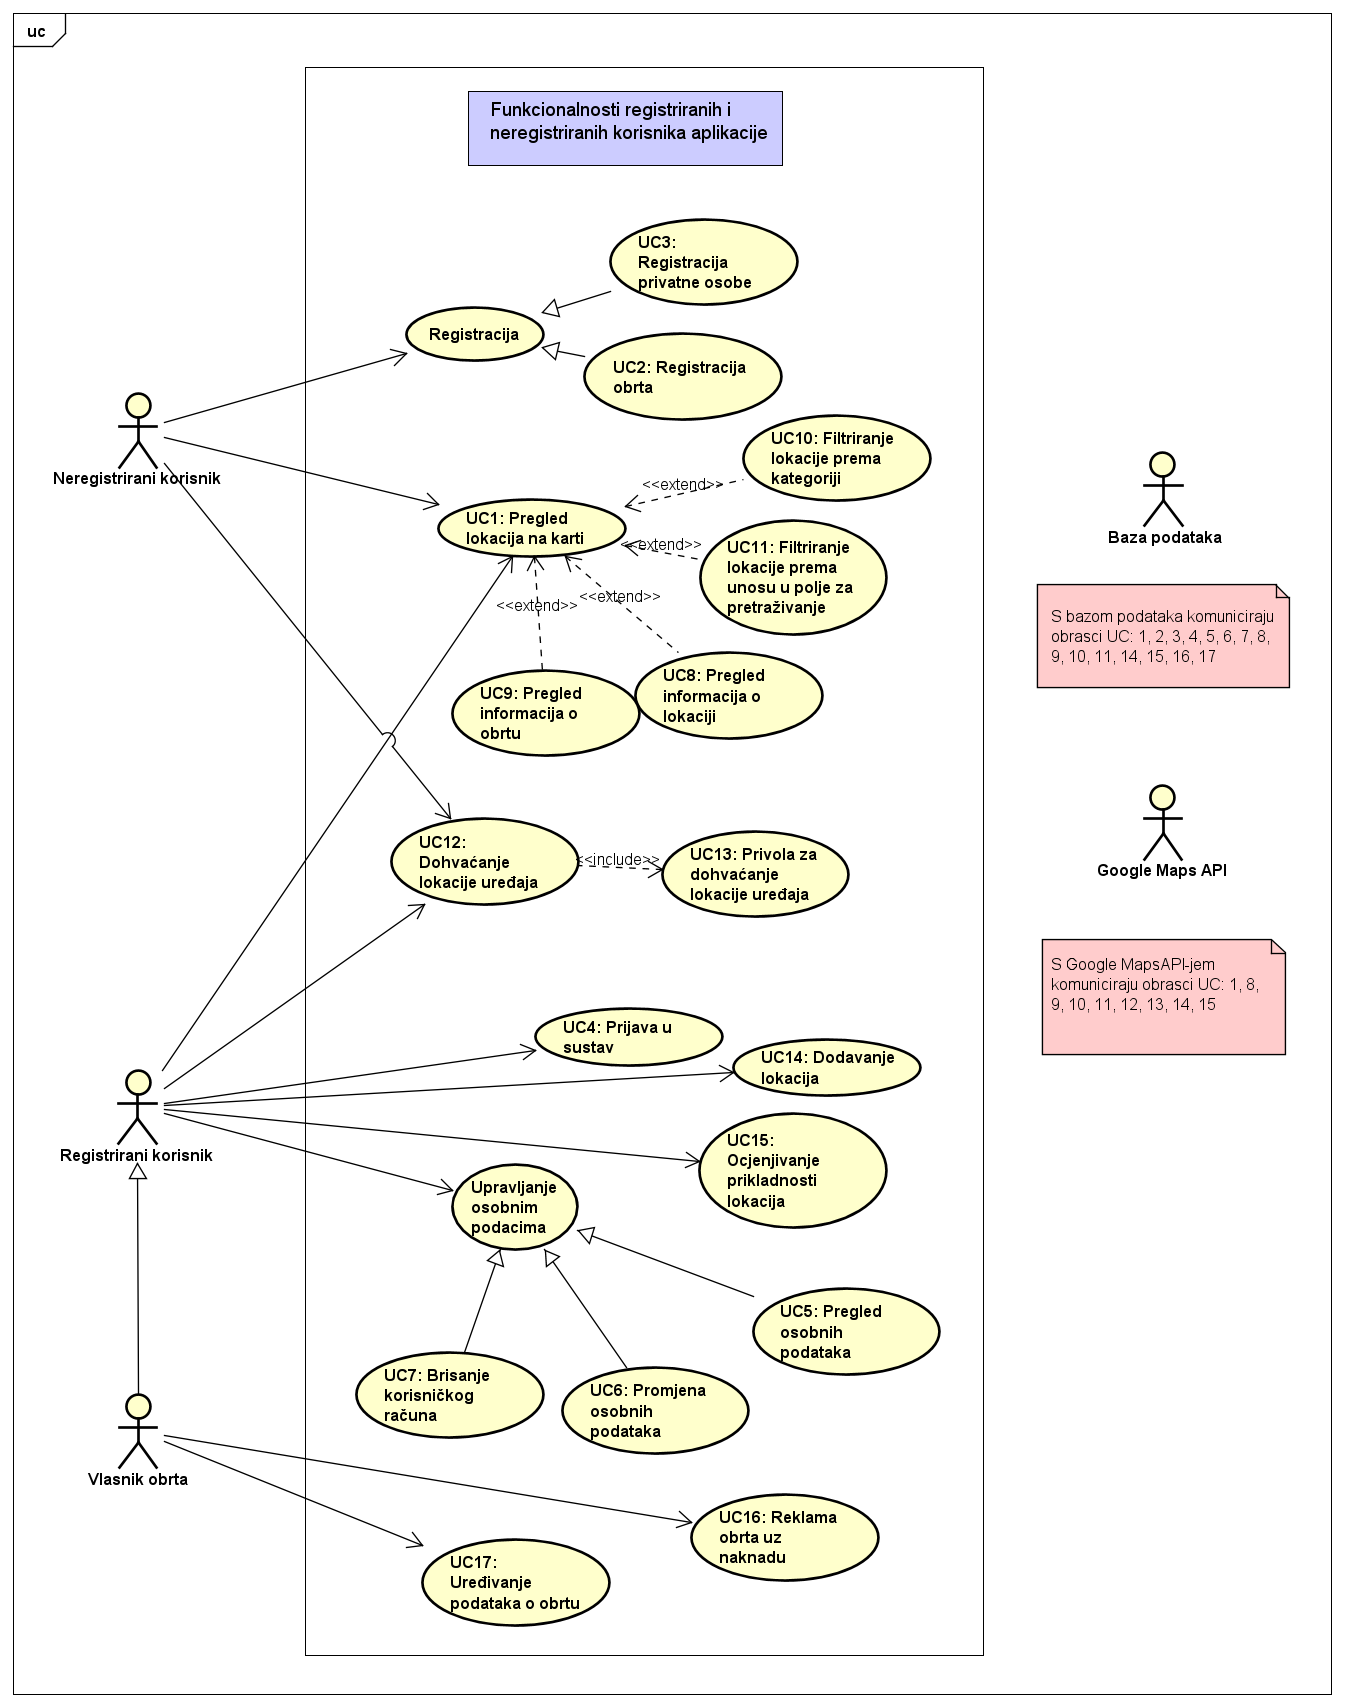
\includegraphics[scale=1.2]{slike/UseCaseDiagram2.png}
						\centering
						\caption{Dijagram obrazaca uporabe}
						\label{fig:promjene}
					\end{figure}
				\eject		
				
			\subsection{Sekvencijski dijagrami}
				
				\textbf{\textit{dio 1. revizije}}\\
				
				\textit{Nacrtati sekvencijske dijagrame koji modeliraju najvažnije dijelove sustava (max. 4 dijagrama). Ukoliko postoji nedoumica oko odabira, razjasniti s asistentom. Uz svaki dijagram napisati detaljni opis dijagrama.}
				\eject
	
		\section{Ostali zahtjevi}
		
			\textbf{\textit{dio 1. revizije}}\\
		 
			 \textit{Nefunkcionalni zahtjevi i zahtjevi domene primjene dopunjuju funkcionalne zahtjeve. Oni opisuju \textbf{kako se sustav treba ponašati} i koja \textbf{ograničenja} treba poštivati (performanse, korisničko iskustvo, pouzdanost, standardi kvalitete, sigurnost...). Primjeri takvih zahtjeva u Vašem projektu mogu biti: podržani jezici korisničkog sučelja, vrijeme odziva, najveći mogući podržani broj korisnika, podržane web/mobilne platforme, razina zaštite (protokoli komunikacije, kriptiranje...)... Svaki takav zahtjev potrebno je navesti u jednoj ili dvije rečenice.}
			 
			 
			 
	